\section{Рабочий проект}
\subsection{Спецификация компонентов и классов программы}

%Описание классов
\subsubsection{Спецификация класса DatabaseConnection}

Данный класс отвечает за создание единственного объекта соединения с базой данной. В таблице \ref{dbp:table} приведена спецификация свойств класса DatabaseConnection.

\renewcommand{\arraystretch}{0.8} % уменьшение расстояний до сетки таблицы
\begin{xltabular}{\textwidth}{|X|p{2.5cm}|>{\setlength{\baselineskip}{0.7\baselineskip}}p{4.85cm}|>{\setlength{\baselineskip}{0.7\baselineskip}}p{4.85cm}|}
	\caption{Спецификация свойств класса DatabaseConnection\label{dbp:table}}\\
	\hline \centrow \setlength{\baselineskip}{0.7\baselineskip} Имя свойства & \centrow \setlength{\baselineskip}{0.7\baselineskip} Область видимости & \centrow Тип данных & \centrow Описание \\
	\hline \centrow 1 & \centrow 2 & \centrow 3 & \centrow 4\\ \hline
	\endfirsthead
%	\caption*{Продолжение таблицы \ref{dbp:table}}\\
	\hline \centrow 1 & \centrow 2 & \centrow 3 & \centrow 4\\ \hline
	\finishhead
	instance & private static & DatabaseConnection & Объект класса DatabaseConnection.\\
	\hline connection & private static & mysqli & Объект подключения к базе данных. 
\end{xltabular}
\renewcommand{\arraystretch}{1.0} % восстановление сетки

В таблице \ref{dbm:table} приведена спецификация методов класса DatabaseConnection.

\renewcommand{\arraystretch}{0.8} % уменьшение расстояний до сетки таблицы
\begin{xltabular}{\textwidth}{|p{2.5cm}|p{2.5cm}|X|>{\setlength{\baselineskip}{0.7\baselineskip}}p{4.85cm}|>{\setlength{\baselineskip}{0.7\baselineskip}}p{4.85cm}|}
	\caption{Спецификация методов класса DatabaseConnection\label{dbm:table}}\\
	\hline \centrow \setlength{\baselineskip}{0.7\baselineskip} Имя  метода & \centrow \setlength{\baselineskip}{0.7\baselineskip} Область видимости & \centrow Описание \\
	\hline \centrow 1 & \centrow 2 & \centrow 3\\ \hline
	\endfirsthead
	\continuecaption{Продолжение таблицы \ref{dbm:table}}
%	\caption*{Продолжение таблицы \ref{dbm:table}}\\
	\hline \centrow 1 & \centrow 2 & \centrow 3\\ \hline
	\finishhead
	getInstance & public static & Возвращает объект класса DatabaseConnection. Если его не существует, он создается.\\
	\hline connect & public & Устанавливает соединение с базой данных, используя предоставленные параметры, и сохраняет объект соединения в свойстве connection.\\
	\hline getConnec\-tion & public & Возвращает текущий объект подключения к базе данных.
\end{xltabular}
\renewcommand{\arraystretch}{1.0} % восстановление сетки

\subsubsection{Спецификация класса Entity}

Данный класс служит базовым классом для представления сущностей базы данных в системе. Он предоставляет основные методы для взаимодействия с базой данных, такие как добавление, обновление, удаление и получение записей. В таблице \ref{entityp:table} приведена спецификация свойств класса Entity.

\renewcommand{\arraystretch}{0.8} % уменьшение расстояний до сетки таблицы
\begin{xltabular}{\textwidth}{|X|p{2.5cm}|>{\setlength{\baselineskip}{0.7\baselineskip}}p{4.85cm}|>{\setlength{\baselineskip}{0.7\baselineskip}}p{4.85cm}|}
	\caption{Спецификация свойств класса Entity\label{entityp:table}}\\
	\hline \centrow \setlength{\baselineskip}{0.7\baselineskip} Имя свойства & \centrow \setlength{\baselineskip}{0.7\baselineskip} Область видимости & \centrow Тип данных & \centrow Описание \\
	\hline \centrow 1 & \centrow 2 & \centrow 3 & \centrow 4\\ \hline
	\endfirsthead
	\continuecaption{Продолжение таблицы \ref{entityp:table}}
%	\caption*{Продолжение таблицы \ref{entityp:table}}\\
	\hline \centrow 1 & \centrow 2 & \centrow 3 & \centrow 4\\ \hline
	\finishhead
	id & protected & int & Уникальный идентификатор сущности.\\
	\hline dbConn & protected & mysqli & Объект подключения к базе данных.\\
	\hline tableName & protected static & string & Название таблицы в базе данных.\\
	\hline fields & protected & array & Массив полей сущности.\\
	\hline primaryKeys & protected & array & Массив первичных ключей.\\
	\hline lastInsertedId & protected & array & Идентификатор последней вставленной записи.
\end{xltabular}
\renewcommand{\arraystretch}{1.0} % восстановление сетки

В таблице \ref{entitym:table} приведена спецификация методов класса Entity.

\renewcommand{\arraystretch}{0.8} % уменьшение расстояний до сетки таблицы
\begin{xltabular}{\textwidth}{|X|p{2.5cm}|>{\setlength{\baselineskip}{0.7\baselineskip}}p{4.85cm}|>{\setlength{\baselineskip}{0.7\baselineskip}}p{4.85cm}|}
	\caption{Спецификация методов класса Entity\label{entitym:table}}\\
	\hline \centrow \setlength{\baselineskip}{0.7\baselineskip} Имя  метода & \centrow \setlength{\baselineskip}{0.7\baselineskip} Область видимости & \centrow Описание \\
	\hline \centrow 1 & \centrow 2 & \centrow 3\\ \hline
	\endfirsthead
	\continuecaption{Продолжение таблицы \ref{entitym:table}}
%	\caption*{Продолжение таблицы \ref{entitym:table}}\\
	\hline \centrow 1 & \centrow 2 & \centrow 3\\ \hline
	\finishhead
	initFields & protected & Абстрактный метод, который реализован в классах-наследниках для инициализации массива fields.\\
	\hline add & public static & Создает объект и новую запись в базе данных, возвращает созданный объект.\\
	\hline update & public & Обновляет текущую запись сущности в базе данных.\\
	\hline getAll & public static & Возвращает массив объектов сущностей, соответствующих условиям выборки.\\
	\hline getByField & public static & Возвращает первый объект, соответствующий полю и его значению.\\
	\hline setFieldValues & protected & Устанавливает значения свойств сущности на основе переданных данных.\\
	\hline insert & protected & Вставляет новую запись в таблицу БД изпользуя значения элементов массива fields.\\
	\hline save & protected & Обновляет запись в БД на основе текущих значений свойств которые соответсвуют элементам массива fields.\\
	\hline delete & public & Удаляет запись из таблицы БД.\\
	\hline getData & private static & Получает данные полученные в результате запроса к БД в виде массива ассоциативных массивов.\\
	\hline getObjects & private static & Получает данные из БД и преобразует их в массив объектов текущего класса.\\
	\hline getType & private static & Определяет тип переданного значения для корректной работы подготовленных запросов.
\end{xltabular}
\renewcommand{\arraystretch}{1.0} % восстановление сетки

\subsubsection{Спецификация класса ContentEntity}

Данный класс расширяющиряет функциональность базового класса Entity и содержит методы для управления маршрутизацией и обработки действий после добавления и обновления данных. В таблице \ref{centityp:table} приведена спецификация свойств класса ContentEntity.

\renewcommand{\arraystretch}{0.8} % уменьшение расстояний до сетки таблицы
\begin{xltabular}{\textwidth}{|X|p{2.5cm}|>{\setlength{\baselineskip}{0.7\baselineskip}}p{4.85cm}|>{\setlength{\baselineskip}{0.7\baselineskip}}p{4.85cm}|}
	\caption{Спецификация свойств класса ContentEntity\label{centityp:table}}\\
	\hline \centrow \setlength{\baselineskip}{0.7\baselineskip} Имя свойства & \centrow \setlength{\baselineskip}{0.7\baselineskip} Область видимости & \centrow Тип данных & \centrow Описание \\
	\hline \centrow 1 & \centrow 2 & \centrow 3 & \centrow 4\\ \hline
	\endfirsthead
%	\caption*{Продолжение таблицы \ref{centityp:table}}\\
	\hline \centrow 1 & \centrow 2 & \centrow 3 & \centrow 4\\ \hline
	\finishhead
	title & public & string & Название.\\
	\hline url & public & string & URL-адрес.\\
	\hline entityName & protected & string & Имя сущности.\\
	\hline controllerName & protected & string & Название контроллера, используется при создании маршрутов.\\
	\hline updateAction & protected & string & Метод контроллера используемое при запросе страницы сайта.
\end{xltabular}
\renewcommand{\arraystretch}{1.0} % восстановление сетки

В таблице \ref{centitypm:table} приведена спецификация методов класса ContentEntity.

\renewcommand{\arraystretch}{0.8} % уменьшение расстояний до сетки таблицы
\begin{xltabular}{\textwidth}{|X|p{2.5cm}|>{\setlength{\baselineskip}{0.7\baselineskip}}p{4.85cm}|>{\setlength{\baselineskip}{0.7\baselineskip}}p{4.85cm}|}
	\caption{Спецификация методов класса ContentEntity\label{centitypm:table}}\\
	\hline \centrow \setlength{\baselineskip}{0.7\baselineskip} Имя  метода & \centrow \setlength{\baselineskip}{0.7\baselineskip} Область видимости & \centrow Описание \\
	\hline \centrow 1 & \centrow 2 & \centrow 3\\ \hline
	\endfirsthead
%	\caption*{Продолжение таблицы \ref{centitypm:table}}\\
	\hline \centrow 1 & \centrow 2 & \centrow 3\\ \hline
	\finishhead
	manageRoute & protected & Обновляет или добавляет маршрут в таблицу routes на основе сгенерированного URL.\\
	\hline afterInsert & protected & Абстрактный метод, который реализован в классах-наследниках. Выполненият действия после добавления объекта.\\
	\hline afterUpdate & protected & Абстрактный метод, который реализован в классах-наследниках. Выполненият действия после обновления объекта.\\
	\hline generateUrl & protected & Генерирует уникальный URL-адрес.
\end{xltabular}
\renewcommand{\arraystretch}{1.0} % восстановление сетки

\subsubsection{Спецификация класса Controller}

Данный класс предназначен для обработки действий пользователя и вызова соответствующего метода в классе наследнике. В таблице \ref{cp:table} приведена спецификация свойств класса Controller.

\renewcommand{\arraystretch}{0.8} % уменьшение расстояний до сетки таблицы
\begin{xltabular}{\textwidth}{|X|p{2.5cm}|>{\setlength{\baselineskip}{0.7\baselineskip}}p{4.85cm}|>{\setlength{\baselineskip}{0.7\baselineskip}}p{4.85cm}|}
	\caption{Спецификация свойств класса Controller\label{cp:table}}\\
	\hline \centrow \setlength{\baselineskip}{0.7\baselineskip} Имя свойства & \centrow \setlength{\baselineskip}{0.7\baselineskip} Область видимости & \centrow Тип данных & \centrow Описание \\
	\hline \centrow 1 & \centrow 2 & \centrow 3 & \centrow 4\\ \hline
	\endfirsthead
%	\caption*{Продолжение таблицы \ref{cp:table}}\\
	\hline \centrow 1 & \centrow 2 & \centrow 3 & \centrow 4\\ \hline
	\finishhead
	dbConn & protected & mysqli & Объект подключения к базе данных.\\
	\hline template & protected & Template & Объект класса Template.
\end{xltabular}
\renewcommand{\arraystretch}{1.0} % восстановление сетки

В таблице \ref{cm:table} приведена спецификация методов класса Controller.

\renewcommand{\arraystretch}{0.8} % уменьшение расстояний до сетки таблицы
\begin{xltabular}{\textwidth}{|X|p{2.5cm}|>{\setlength{\baselineskip}{0.7\baselineskip}}p{4.85cm}|>{\setlength{\baselineskip}{0.7\baselineskip}}p{4.85cm}|}
	\caption{Спецификация методов класса Controller\label{cm:table}}\\
	\hline \centrow \setlength{\baselineskip}{0.7\baselineskip} Имя  метода & \centrow \setlength{\baselineskip}{0.7\baselineskip} Область видимости & \centrow Описание \\
	\hline \centrow 1 & \centrow 2 & \centrow 3\\ \hline
	\endfirsthead
%	\caption*{Продолжение таблицы \ref{cm:table}}\\
	\hline \centrow 1 & \centrow 2 & \centrow 3\\ \hline
	\finishhead
	runAction & public & Вызывает метод контроллера, соответствующей переданному названию.
\end{xltabular}
\renewcommand{\arraystretch}{1.0} % восстановление сетки

\subsubsection{Спецификация класса Template}

Данный класс используется для управления отображением представлений используя определнный шаблон. В таблице \ref{templatep:table} приведена спецификация свойств класса Template.

\renewcommand{\arraystretch}{0.8} % уменьшение расстояний до сетки таблицы
\begin{xltabular}{\textwidth}{|X|p{2.5cm}|>{\setlength{\baselineskip}{0.7\baselineskip}}p{4.85cm}|>{\setlength{\baselineskip}{0.7\baselineskip}}p{4.85cm}|}
	\caption{Спецификация свойств класса Template\label{templatep:table}}\\
	\hline \centrow \setlength{\baselineskip}{0.7\baselineskip} Имя свойства & \centrow \setlength{\baselineskip}{0.7\baselineskip} Область видимости & \centrow Тип данных & \centrow Описание \\
	\hline \centrow 1 & \centrow 2 & \centrow 3 & \centrow 4\\ \hline
	\endfirsthead
%	\caption*{Продолжение таблицы \ref{templatep:table}}\\
	\hline \centrow 1 & \centrow 2 & \centrow 3 & \centrow 4\\ \hline
	\finishhead
	templatePath & private & string & Путь к файлу шаблона, который будет использоваться для отображения представления.\\
	\hline context & private & string & Контекст использования шаблона.\\
	\hline dbConn & private & mysqli & Объект подключения к базе данных.
\end{xltabular}
\renewcommand{\arraystretch}{1.0} % восстановление сетки

В таблице \ref{templatem:table} приведена спецификация методов класса Template.

\renewcommand{\arraystretch}{0.8} % уменьшение расстояний до сетки таблицы
\begin{xltabular}{\textwidth}{|X|p{2.5cm}|>{\setlength{\baselineskip}{0.7\baselineskip}}p{4.85cm}|>{\setlength{\baselineskip}{0.7\baselineskip}}p{4.85cm}|}
	\caption{Спецификация методов класса Template\label{templatem:table}}\\
	\hline \centrow \setlength{\baselineskip}{0.7\baselineskip} Имя  метода & \centrow \setlength{\baselineskip}{0.7\baselineskip} Область видимости & \centrow Описание \\
	\hline \centrow 1 & \centrow 2 & \centrow 3\\ \hline
	\endfirsthead
%	\caption*{Продолжение таблицы \ref{templatem:table}}\\
	\hline \centrow 1 & \centrow 2 & \centrow 3\\ \hline
	\finishhead
	renderView & public & Отображает переданное представление в определенном шаблоне.
\end{xltabular}
\renewcommand{\arraystretch}{1.0} % восстановление сетки

\subsubsection{Спецификация класса Page}

Данный класс представляет модель страницы. Этот класс наследует функциональность класса ContentEntity и содержит методы для управления иерархией страниц и обновлением пунктов меню. В таблице \ref{pagep:table} приведена спецификация свойств класса Page.

\renewcommand{\arraystretch}{0.8} % уменьшение расстояний до сетки таблицы
\begin{xltabular}{\textwidth}{|X|p{2.5cm}|>{\setlength{\baselineskip}{0.7\baselineskip}}p{4.85cm}|>{\setlength{\baselineskip}{0.7\baselineskip}}p{4.85cm}|}
	\caption{Спецификация свойств класса Page\label{pagep:table}}\\
	\hline \centrow \setlength{\baselineskip}{0.7\baselineskip} Имя свойства & \centrow \setlength{\baselineskip}{0.7\baselineskip} Область видимости & \centrow Тип данных & \centrow Описание \\
	\hline \centrow 1 & \centrow 2 & \centrow 3 & \centrow 4\\ \hline
	\endfirsthead
%	\caption*{Продолжение таблицы \ref{pagep:table}}\\
	\hline \centrow 1 & \centrow 2 & \centrow 3 & \centrow 4\\ \hline
	\finishhead
	content & public & string & Содержимое страницы.\\
	\hline parent\_page\_id & public & int & Идентификатор родительской страницы.
\end{xltabular}
\renewcommand{\arraystretch}{1.0} % восстановление сетки

В таблице \ref{pagem:table} приведена спецификация методов класса Page.

\renewcommand{\arraystretch}{0.8} % уменьшение расстояний до сетки таблицы
\begin{xltabular}{\textwidth}{|X|p{2.5cm}|>{\setlength{\baselineskip}{0.7\baselineskip}}p{4.85cm}|>{\setlength{\baselineskip}{0.7\baselineskip}}p{4.85cm}|}
	\caption{Спецификация методов класса Page\label{pagem:table}}\\
	\hline \centrow \setlength{\baselineskip}{0.7\baselineskip} Имя  метода & \centrow \setlength{\baselineskip}{0.7\baselineskip} Область видимости & \centrow Описание \\
	\hline \centrow 1 & \centrow 2 & \centrow 3\\ \hline
	\endfirsthead
%	\caption*{Продолжение таблицы \ref{pagem:table}}\\
	\hline \centrow 1 & \centrow 2 & \centrow 3\\ \hline
	\finishhead
	updateMenuItems & private & Обновляет URL-адреса в элементах меню, связанных с текущей страницей.\\
	\hline getChildPages & public & Возвращает массив объектов Page, представляющих дочерние страницы.
\end{xltabular}
\renewcommand{\arraystretch}{1.0} % восстановление сетки

\subsubsection{Спецификация класса Post}

Данный класс представляет модель поста. Этот класс наследует функциональность класса ContentEntity и содержит методы для управления категориями постов. В таблице \ref{postp:table} приведена спецификация свойств класса Post.

\renewcommand{\arraystretch}{0.8} % уменьшение расстояний до сетки таблицы
\begin{xltabular}{\textwidth}{|X|p{2.5cm}|>{\setlength{\baselineskip}{0.7\baselineskip}}p{4.85cm}|>{\setlength{\baselineskip}{0.7\baselineskip}}p{4.85cm}|}
	\caption{Спецификация свойств класса Post\label{postp:table}}\\
	\hline \centrow \setlength{\baselineskip}{0.7\baselineskip} Имя свойства & \centrow \setlength{\baselineskip}{0.7\baselineskip} Область видимости & \centrow Тип данных & \centrow Описание \\
	\hline \centrow 1 & \centrow 2 & \centrow 3 & \centrow 4\\ \hline
	\endfirsthead
%	\caption*{Продолжение таблицы \ref{postp:table}}\\
	\hline \centrow 1 & \centrow 2 & \centrow 3 & \centrow 4\\ \hline
	\finishhead
	content & public & string & Содержимое поста.\\
	\hline author\_id & public & int & Идентификатор автора поста.\\
	\hline author & public & User & Объект автора поста.\\
	\hline updated\_datetime & public & Date & Дата и время последнего обновления поста.\\
	\hline categories & public & array & Список категорий, к которым относится пост.
\end{xltabular}
\renewcommand{\arraystretch}{1.0} % восстановление сетки

В таблице \ref{postm:table} приведена спецификация методов класса Post.

\renewcommand{\arraystretch}{0.8} % уменьшение расстояний до сетки таблицы
\begin{xltabular}{\textwidth}{|X|p{2.5cm}|>{\setlength{\baselineskip}{0.7\baselineskip}}p{4.85cm}|>{\setlength{\baselineskip}{0.7\baselineskip}}p{4.85cm}|}
	\caption{Спецификация методов класса Post\label{postm:table}}\\
	\hline \centrow \setlength{\baselineskip}{0.7\baselineskip} Имя  метода & \centrow \setlength{\baselineskip}{0.7\baselineskip} Область видимости & \centrow Описание \\
	\hline \centrow 1 & \centrow 2 & \centrow 3\\ \hline
	\endfirsthead
%	\caption*{Продолжение таблицы \ref{postm:table}}\\
	\hline \centrow 1 & \centrow 2 & \centrow 3\\ \hline
	\finishhead
	updatePostCategories & private & Обновляет категории поста в базе данных. Удаляет текущие категории и добавляет новые.\\
	\hline getCategories & public & Возвращает массив объектов Category, к которым относится пост.\\
	\hline getCategoryIds & public & Возвращает массив идентификаторов категорий, к которым относится пост.\\
	\hline getPostsByCategory & private & Возвращает массив объектов Post, которые относятся к указанной категории.
\end{xltabular}
\renewcommand{\arraystretch}{1.0} % восстановление сетки

\subsubsection{Спецификация класса Category}

Данный класс представляет модель категории. Этот класс наследует функциональность класса ContentEntity и содержит основные методы для управления категориями постов. В таблице \ref{catp:table} приведена спецификация свойств класса Category.

\renewcommand{\arraystretch}{0.8} % уменьшение расстояний до сетки таблицы
\begin{xltabular}{\textwidth}{|X|p{2.5cm}|>{\setlength{\baselineskip}{0.7\baselineskip}}p{4.85cm}|>{\setlength{\baselineskip}{0.7\baselineskip}}p{4.85cm}|}
	\caption{Спецификация свойств класса Category\label{catp:table}}\\
	\hline \centrow \setlength{\baselineskip}{0.7\baselineskip} Имя свойства & \centrow \setlength{\baselineskip}{0.7\baselineskip} Область видимости & \centrow Тип данных & \centrow Описание \\
	\hline \centrow 1 & \centrow 2 & \centrow 3 & \centrow 4\\ \hline
	\endfirsthead
%	\caption*{Продолжение таблицы \ref{catp:table}}\\
	\hline \centrow 1 & \centrow 2 & \centrow 3 & \centrow 4\\ \hline
	\finishhead
	parent\_category\_id & public & int & Идентификатор родительской категории.
\end{xltabular}
\renewcommand{\arraystretch}{1.0} % восстановление сетки

В таблице \ref{catm:table} приведена спецификация методов класса Category.

\renewcommand{\arraystretch}{0.8} % уменьшение расстояний до сетки таблицы
\begin{xltabular}{\textwidth}{|X|p{2.5cm}|>{\setlength{\baselineskip}{0.7\baselineskip}}p{4.85cm}|>{\setlength{\baselineskip}{0.7\baselineskip}}p{4.85cm}|}
	\caption{Спецификация методов класса Category\label{catm:table}}\\
	\hline \centrow \setlength{\baselineskip}{0.7\baselineskip} Имя  метода & \centrow \setlength{\baselineskip}{0.7\baselineskip} Область видимости & \centrow Описание \\
	\hline \centrow 1 & \centrow 2 & \centrow 3\\ \hline
	\endfirsthead
%	\caption*{Продолжение таблицы \ref{catm:table}}\\
	\hline \centrow 1 & \centrow 2 & \centrow 3\\ \hline
	\finishhead
	getChildCategories & public & Возвращает массив объектов дочерних категорий.
\end{xltabular}
\renewcommand{\arraystretch}{1.0} % восстановление сетки

\subsubsection{Спецификация класса Menu}

Данный класс представляет модель меню. Этот класс наследует функциональность класса Entity и содержит основные методы для управления областями меню и пунктами меню. В таблице \ref{menup:table} приведена спецификация свойств класса Menu.

\renewcommand{\arraystretch}{0.8} % уменьшение расстояний до сетки таблицы
\begin{xltabular}{\textwidth}{|X|p{2.5cm}|>{\setlength{\baselineskip}{0.7\baselineskip}}p{4.85cm}|>{\setlength{\baselineskip}{0.7\baselineskip}}p{4.85cm}|}
	\caption{Спецификация свойств класса Category\label{menup:table}}\\
	\hline \centrow \setlength{\baselineskip}{0.7\baselineskip} Имя свойства & \centrow \setlength{\baselineskip}{0.7\baselineskip} Область видимости & \centrow Тип данных & \centrow Описание \\
	\hline \centrow 1 & \centrow 2 & \centrow 3 & \centrow 4\\ \hline
	\endfirsthead
%	\caption*{Продолжение таблицы \ref{menup:table}}\\
	\hline \centrow 1 & \centrow 2 & \centrow 3 & \centrow 4\\ \hline
	\finishhead
	name & public & string & Название области меню.
\end{xltabular}
\renewcommand{\arraystretch}{1.0} % восстановление сетки

В таблице \ref{catm:table} приведена спецификация методов класса Menu.

\renewcommand{\arraystretch}{0.8} % уменьшение расстояний до сетки таблицы
\begin{xltabular}{\textwidth}{|X|p{2.5cm}|>{\setlength{\baselineskip}{0.7\baselineskip}}p{4.85cm}|>{\setlength{\baselineskip}{0.7\baselineskip}}p{4.85cm}|}
	\caption{Спецификация методов класса Menu\label{menum:table}}\\
	\hline \centrow \setlength{\baselineskip}{0.7\baselineskip} Имя  метода & \centrow \setlength{\baselineskip}{0.7\baselineskip} Область видимости & \centrow Описание \\
	\hline \centrow 1 & \centrow 2 & \centrow 3\\ \hline
	\endfirsthead
%	\caption*{Продолжение таблицы \ref{menum:table}}\\
	\hline \centrow 1 & \centrow 2 & \centrow 3\\ \hline
	\finishhead
	getMenuItems & public & Возвращает массив объектов элементов меню.\\
	\hline getAddedPageIds & public & Возвращает массив идентификаторов страниц, которые были добавлены в меню.\\
	\hline getNextOrderNum & private & Возвращает следующий порядковый номер для нового элемента меню в текущем меню.\\
	\hline addMenuItem & public & Добавляет новый элемент меню в текущее меню.\\
	\hline updateMenuItemsOrder & public & Обновляет порядок элементов меню согласно новому порядку элементов.\\
\end{xltabular}
\renewcommand{\arraystretch}{1.0} % восстановление сетки

\subsubsection{Спецификация класса Route}

Данный класс представляет модель маршрут. Он связывает URL-адреса с методами контроллеров. В таблице \ref{routep:table} приведена спецификация свойств класса Route.

\renewcommand{\arraystretch}{0.8} % уменьшение расстояний до сетки таблицы
\begin{xltabular}{\textwidth}{|X|p{2.5cm}|>{\setlength{\baselineskip}{0.7\baselineskip}}p{4.85cm}|>{\setlength{\baselineskip}{0.7\baselineskip}}p{4.85cm}|}
	\caption{Спецификация свойств класса Route\label{routep:table}}\\
	\hline \centrow \setlength{\baselineskip}{0.7\baselineskip} Имя свойства & \centrow \setlength{\baselineskip}{0.7\baselineskip} Область видимости & \centrow Тип данных & \centrow Описание \\
	\hline \centrow 1 & \centrow 2 & \centrow 3 & \centrow 4\\ \hline
	\endfirsthead
	%	\caption*{Продолжение таблицы \ref{routep:table}}\\
	\hline \centrow 1 & \centrow 2 & \centrow 3 & \centrow 4\\ \hline
	\finishhead
	path & public & string & URL-адрес.\\
	\hline controller & public & string & Название контроллера связанного с маршрутом.\\
	\hline action & public & string & Метод контроллера связанного с маршрутом.\\
	\hline page\_id & public & int & Идентификатор связанной страницы.\\
	\hline post\_id & public & int & Идентификатор связанного поста.\\
	\hline category\_id & public & int & Идентификатор связанной категории.\\
	\hline tag\_id & public & int & Идентификатор связанного тега.
\end{xltabular}
\renewcommand{\arraystretch}{1.0} % восстановление сетки

В таблице \ref{routem:table} приведена спецификация методов класса Route.

\renewcommand{\arraystretch}{0.8} % уменьшение расстояний до сетки таблицы
\begin{xltabular}{\textwidth}{|X|p{2.5cm}|>{\setlength{\baselineskip}{0.7\baselineskip}}p{4.85cm}|>{\setlength{\baselineskip}{0.7\baselineskip}}p{4.85cm}|}
	\caption{Спецификация методов класса Route\label{routem:table}}\\
	\hline \centrow \setlength{\baselineskip}{0.7\baselineskip} Имя  метода & \centrow \setlength{\baselineskip}{0.7\baselineskip} Область видимости & \centrow Описание \\
	\hline \centrow 1 & \centrow 2 & \centrow 3\\ \hline
	\endfirsthead
	%	\caption*{Продолжение таблицы \ref{routem:table}}\\
	\hline \centrow 1 & \centrow 2 & \centrow 3\\ \hline
	\finishhead
	add & public static &  Создает новый маршрут в базе данных, используя переданные данные.\\
	\hline updatePath & public & Обновляет поле path маршрута и сохраняет изменения в БД.
\end{xltabular}
\renewcommand{\arraystretch}{1.0} % восстановление сетки

\subsubsection{Спецификация класса PageController}

Данный класс предназначен для управления страницами в административной панели. В таблице \ref{pgc:table} приведена спецификация методов класса PageController.

\renewcommand{\arraystretch}{0.8} % уменьшение расстояний до сетки таблицы
\begin{xltabular}{\textwidth}{|X|p{2.5cm}|>{\setlength{\baselineskip}{0.7\baselineskip}}p{4.85cm}|>{\setlength{\baselineskip}{0.7\baselineskip}}p{4.85cm}|}
	\caption{Спецификация методов класса PageController\label{pgc:table}}\\
	\hline \centrow \setlength{\baselineskip}{0.7\baselineskip} Имя  метода & \centrow \setlength{\baselineskip}{0.7\baselineskip} Область видимости & \centrow Описание \\
	\hline \centrow 1 & \centrow 2 & \centrow 3\\ \hline
	\endfirsthead
%	\caption*{Продолжение таблицы \ref{pgc:table}}\\
	\hline \centrow 1 & \centrow 2 & \centrow 3\\ \hline
	\finishhead
	defaultAction & public & Отображает список страниц в административной панели. Получает все страницы из БД и передает их в представление для отображения.\\
	\hline editPageAction & public & Обрабатывает обновление страницы. Загружает данные страницы, и отображает форму редактирования.\\
	\hline addPageAction & public & Обрабатывает добавление новой страницы. Отображает форму для добавления новой страницы.\\
	\hline deletePageAction & public & Обрабатывает удаление страницы.
\end{xltabular}
\renewcommand{\arraystretch}{1.0} % восстановление сетки

\subsubsection{Спецификация класса PostController}

Данный класс предназначен для управления постами в административной панели. В таблице \ref{pstc:table} приведена спецификация методов класса PostController.

\renewcommand{\arraystretch}{0.8} % уменьшение расстояний до сетки таблицы
\begin{xltabular}{\textwidth}{|X|p{2.5cm}|>{\setlength{\baselineskip}{0.7\baselineskip}}p{4.85cm}|>{\setlength{\baselineskip}{0.7\baselineskip}}p{4.85cm}|}
	\caption{Спецификация методов класса PostController\label{pstc:table}}\\
	\hline \centrow \setlength{\baselineskip}{0.7\baselineskip} Имя  метода & \centrow \setlength{\baselineskip}{0.7\baselineskip} Область видимости & \centrow Описание \\
	\hline \centrow 1 & \centrow 2 & \centrow 3\\ \hline
	\endfirsthead
%	\caption*{Продолжение таблицы \ref{pstc:table}}\\
	\hline \centrow 1 & \centrow 2 & \centrow 3\\ \hline
	\finishhead
	defaultAction & public & Отображает список постов в административной панели. Получает все посты из БД и передает их в представление для отображения.\\
	\hline editPostAction & public & Обрабатывает обновление поста. Загружает данные поста, и отображает форму редактирования.\\
	\hline addPostAction & public & Обрабатывает добавление нового поста. Отображает форму для добавления нового поста.\\
	\hline deletePostAction & public & Обрабатывает удаление поста.
\end{xltabular}
\renewcommand{\arraystretch}{1.0} % восстановление сетки

\subsubsection{Спецификация класса MenuController}

Данный класс предназначен для управления областями и пунктами меню. В таблице \ref{menuc:table} приведена спецификация методов класса MenuController.

\renewcommand{\arraystretch}{0.8} % уменьшение расстояний до сетки таблицы
\begin{xltabular}{\textwidth}{|X|p{2.5cm}|>{\setlength{\baselineskip}{0.7\baselineskip}}p{4.85cm}|>{\setlength{\baselineskip}{0.7\baselineskip}}p{4.85cm}|}
	\caption{Спецификация методов класса MenuController\label{menuc:table}}\\
	\hline \centrow \setlength{\baselineskip}{0.7\baselineskip} Имя метода & \centrow \setlength{\baselineskip}{0.7\baselineskip} Область видимости & \centrow Описание \\
	\hline \centrow 1 & \centrow 2 & \centrow 3\\ \hline
	\endfirsthead
%	\caption*{Продолжение таблицы \ref{menuc:table}}\\
	\hline \centrow 1 & \centrow 2 & \centrow 3\\ \hline
	\finishhead
	defaultAction & public & Отображает список областей меню в административной панели. Получает все меню из БД и передает их в представление для отображения.\\
	\hline editMenuAction & public & Обрабатывает редактирование области меню. Загружает данные меню и его элементов, и отображает их в виде списка.\\
	\hline editMenuItemAction & public & Обрабатывает обновление элемента меню меню. Загружает данные элемента меню, и отображает форму редактирования.\\
	\hline addMenuItemAction & public & Обрабатывает добавление нового элемента меню. Отображает форму для добавления элемента меню.\\
	\hline deleteMenuItemAction & public & Обрабатывает удаление элемента меню.\\
	\hline updateMenuOrderAction & public & Обновляет порядок элементов меню.\\
\end{xltabular}
\renewcommand{\arraystretch}{1.0} % восстановление сетки

\subsubsection{Спецификация класса UserController}

Данный класс предназначен для управления пользователями. В таблице \ref{userc:table} приведена спецификация методов класса UserController.

\renewcommand{\arraystretch}{0.8} % уменьшение расстояний до сетки таблицы
\begin{xltabular}{\textwidth}{|X|p{2.5cm}|>{\setlength{\baselineskip}{0.7\baselineskip}}p{4.85cm}|>{\setlength{\baselineskip}{0.7\baselineskip}}p{4.85cm}|}
	\caption{Спецификация методов класса MenuController\label{userc:table}}\\
	\hline \centrow \setlength{\baselineskip}{0.7\baselineskip} Имя метода & \centrow \setlength{\baselineskip}{0.7\baselineskip} Область видимости & \centrow Описание \\
	\hline \centrow 1 & \centrow 2 & \centrow 3\\ \hline
	\endfirsthead
	%	\caption*{Продолжение таблицы \ref{userc:table}}\\
	\hline \centrow 1 & \centrow 2 & \centrow 3\\ \hline
	\finishhead
	defaultAction & public & Отображает список пользователей в административной панели. Получает всех пользователей из БД и передает их в представление для отображения.\\
	\hline editUserAction & public & Обрабатывает редактирование информации о пользователе. Загружает данные о пользователе, и отображает форму редактирования.\\
	\hline addMenuItemAction & public & Обрабатывает добавление нового пользователя. Отображает форму для добавления пользователя.\\
	\hline deleteMenuItemAction & public & Обрабатывает удаление пользователя.\\
\end{xltabular}
\renewcommand{\arraystretch}{1.0} % восстановление сетки

\subsection{Тестирование программной системы}
\subsubsection{Модульное тестирование системы}

Модульный тест для класса Entity представлен на рисунках \ref{unitEntity1:image} -  \ref{unitEntity2:image}.

\begin{figure}[H]
\begin{lstlisting}[language=PHP]
declare(strict_types=1);

use PHPUnit\Framework\TestCase;
use src\Entity;

class User extends Entity
{
	public string $name;
	public string $email;
	protected static string $tableName = 'users';
	
	protected function initFields(): void
	{
		$this->fields = ['name', 'email'];
	}
}

class EntityTest extends TestCase
{
	private $dbConn;
	
	protected function setUp(): void
	{
		$this->dbConn = new mysqli('localhost', 'root', '', 'test_db');
		
		$this->dbConn->query("
			CREATE TABLE IF NOT EXISTS users (
			id INT AUTO_INCREMENT PRIMARY KEY,
			name VARCHAR(255) NOT NULL,
			email VARCHAR(255) NOT NULL
			)
		");
	}
	
	protected function tearDown(): void
	{
		$this->dbConn->query("DROP TABLE IF EXISTS users");
		$this->dbConn->close();
	}
	
	public function testAdd(): void
	{
		$data = ['name' => 'John Doe', 'email' => 'john@example.com'];
		$user = User::add($this->dbConn, $data);
		
		$this->assertInstanceOf(User::class, $user);
		$this->assertEquals('John Doe', $user->name);
		$this->assertEquals('john@example.com', $user->email);
		$this->assertNotNull($user->id);
	}
\end{lstlisting}  
\caption{Модульный тест класса Entity}
\label{unitEntity1:image}
\end{figure}

\begin{figure}[H]
\begin{lstlisting}[language=PHP]
	public function testUpdate(): void
	{
		$data = ['name' => 'John Doe', 'email' => 'john@example.com'];
		$user = User::add($this->dbConn, $data);
		$user->update(['name' => 'Jane Doe']);
		
		$updatedUser = User::getByField($this->dbConn, 'id', $user->id);
		$this->assertEquals('Jane Doe', $updatedUser->name);
	}
	
	public function testGetAll(): void
	{
		User::add($this->dbConn, ['name' => 'John Doe', 'email' => 'john@example.com']);
		User::add($this->dbConn, ['name' => 'Jane Doe', 'email' => 'jane@example.com']);
		
		$users = User::getAll($this->dbConn);
		
		$this->assertCount(2, $users);
	}
	
	public function testGetByField(): void
	{
		$user = User::add($this->dbConn, ['name' => 'John Doe', 'email' => 'john@example.com']);
		
		$retrievedUser = User::getByField($this->dbConn, 'email', 'john@example.com');
		$this->assertInstanceOf(User::class, $retrievedUser);
		$this->assertEquals('John Doe', $retrievedUser->name);
	}
	
	public function testDelete(): void
	{
		$user = User::add($this->dbConn, ['name' => 'John Doe', 'email' => 'john@example.com']);
		$user->delete();
		
		$deletedUser = User::getByField($this->dbConn, 'id', $user->id);
		$this->assertNull($deletedUser);
	}
}
\end{lstlisting}  
\caption{Модульный тест класса Entity}
\label{unitEntity2:image}
\end{figure}

Результаты модульного тестирования класса Entity представлены на рисунке \ref{unit1:image}.

\begin{figure}[H]
	\center{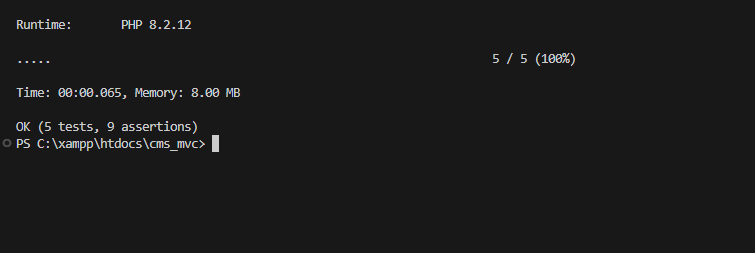
\includegraphics[width=1\linewidth]{unit1}}
	\caption{Результаты модульного тестирования}
	\label{unit1:image}
\end{figure}

\subsubsection{Системное тестирование программной системы}

Для проверки работоспособности разработанной программы было выпоненно системное тестирование. Результаты тестирования представленны в виде снимков экрана.

На рисунке \ref{ui7:image} представлена страница входа в административную панель сайта, которое открывается при запросе из адресной строки браузера. При успешной авторизации пользователь переходит на главную страницу панели и боковое меню для перемещения по соответствующим разделам панели.

\begin{figure}[H]
	\center{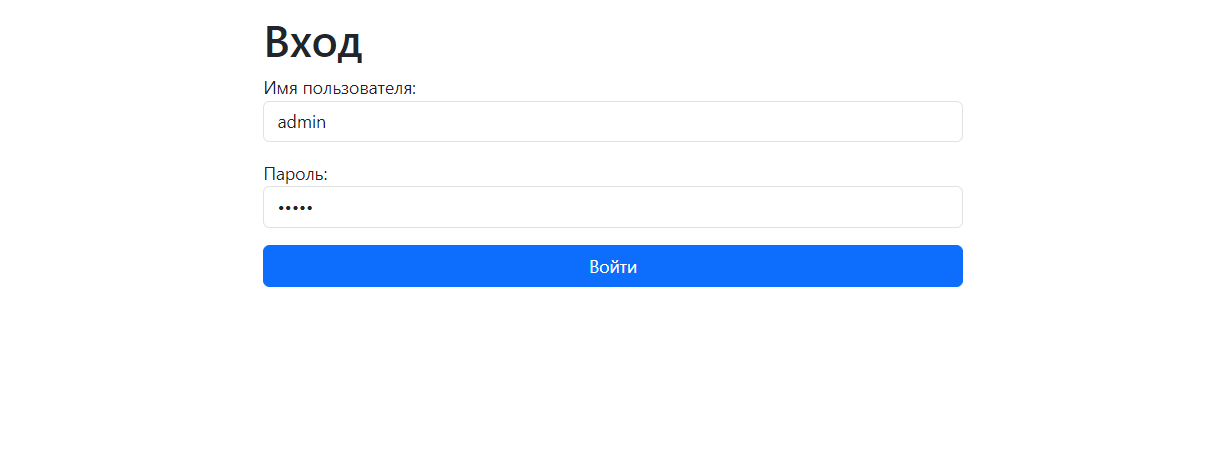
\includegraphics[width=1\linewidth]{ui7}}
	\caption{Страница для входа в административную панель}
	\label{ui7:image}
\end{figure}

%Раздел "<Пользователь"> представляет функции для управления пользователями ситемы, в этом разделе отображается список пользователей \ref{main:image}, кнопки для перехода к форме добавления \ref{main:image} и редактивания \ref{main:image} пользователя.
%
%Раздел "<Страницы"> представляет функции для управления страницами сайта, в этом разделе отображается список страниц сайта \ref{main:image}, кнопки для перехода к форме добавления \ref{main:image} и редактору \ref{main:image} контента.

Для того чтобы управлять страницами сайта, пользователю необходимо перейти в раздел "<Страницы"> (рис. \ref{ui8:image}), в котором отобразиться список страниц сайта. 

\begin{figure}[H]
	\center{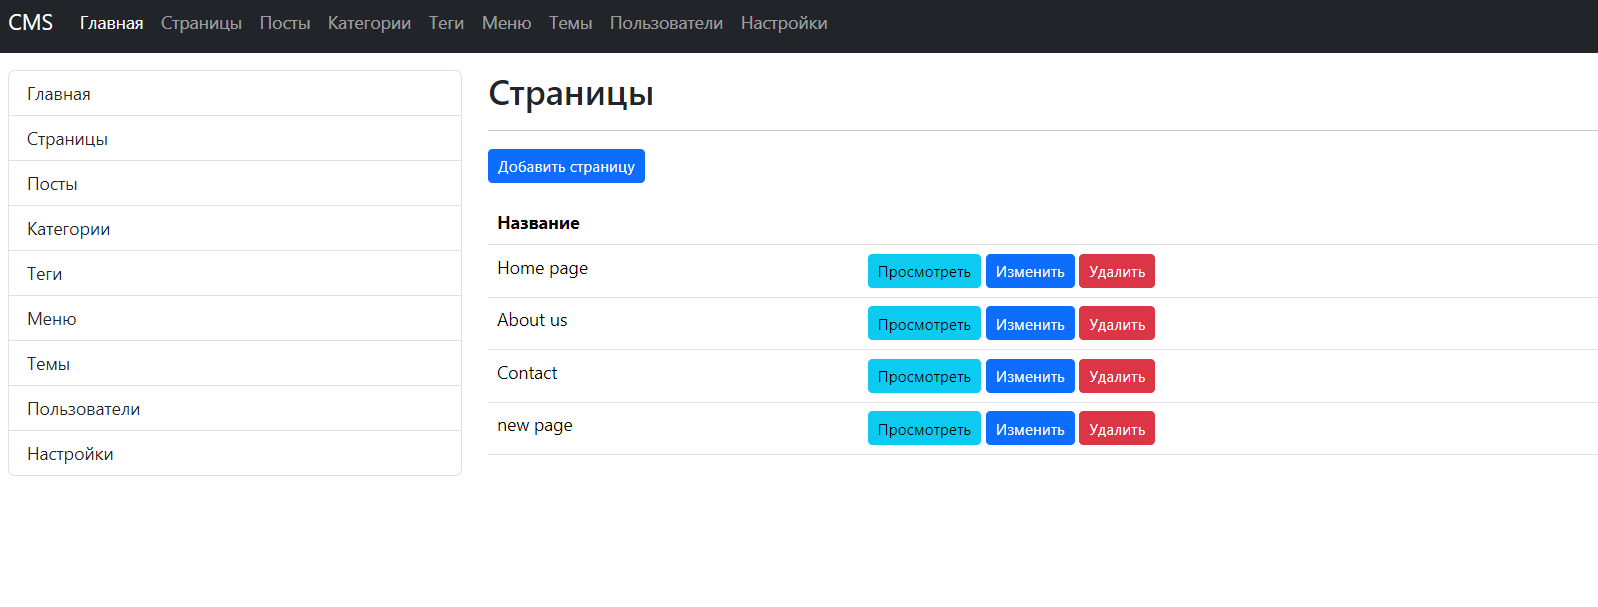
\includegraphics[width=1\linewidth]{ui8}}
	\caption{Список страниц сайта}
	\label{ui8:image}
\end{figure}

Для добавление новой страницы пользователь нажимает на кнопку "<Добавить страницу">, которая открывает форму добавления новой страницы (рис. \ref{ui9:image}). После ввода данных странцы, при нажатии на кнопку "<Добавить">, новая страница добаляется на сайт.

\begin{figure}[H]
	\center{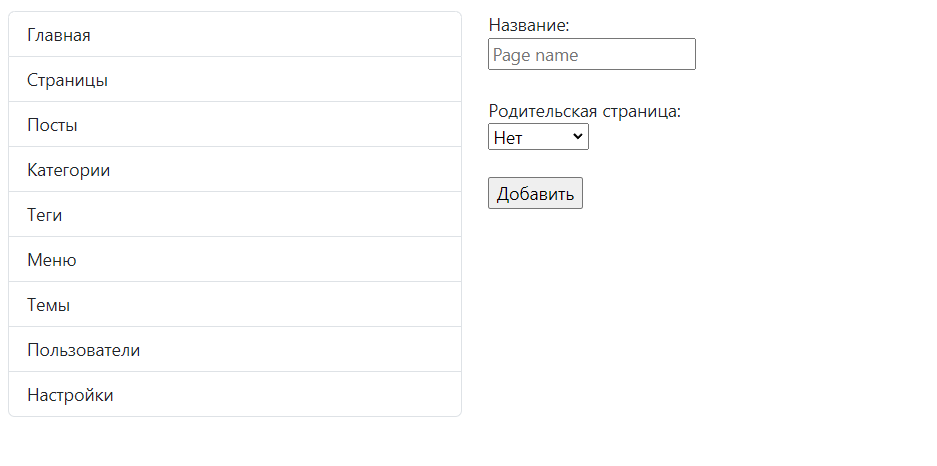
\includegraphics[width=1\linewidth]{ui9}}
	\caption{Форма добавления страницы}
	\label{ui9:image}
\end{figure}

Для редактирования страницы пользователь выбирает страницу из списка страниц и нажимает на кнопку "<Редактировать">, открывается редактор контента (рис. \ref{ui10:image}), в котором пользователь может вносить изменения в содержимое страницы, добавлять различные элементы интерфейса, форматировать текст и др. Для сохранения изменений пользователь нажимает на кнопку "<Сохранить">.

\begin{figure}[H]
	\center{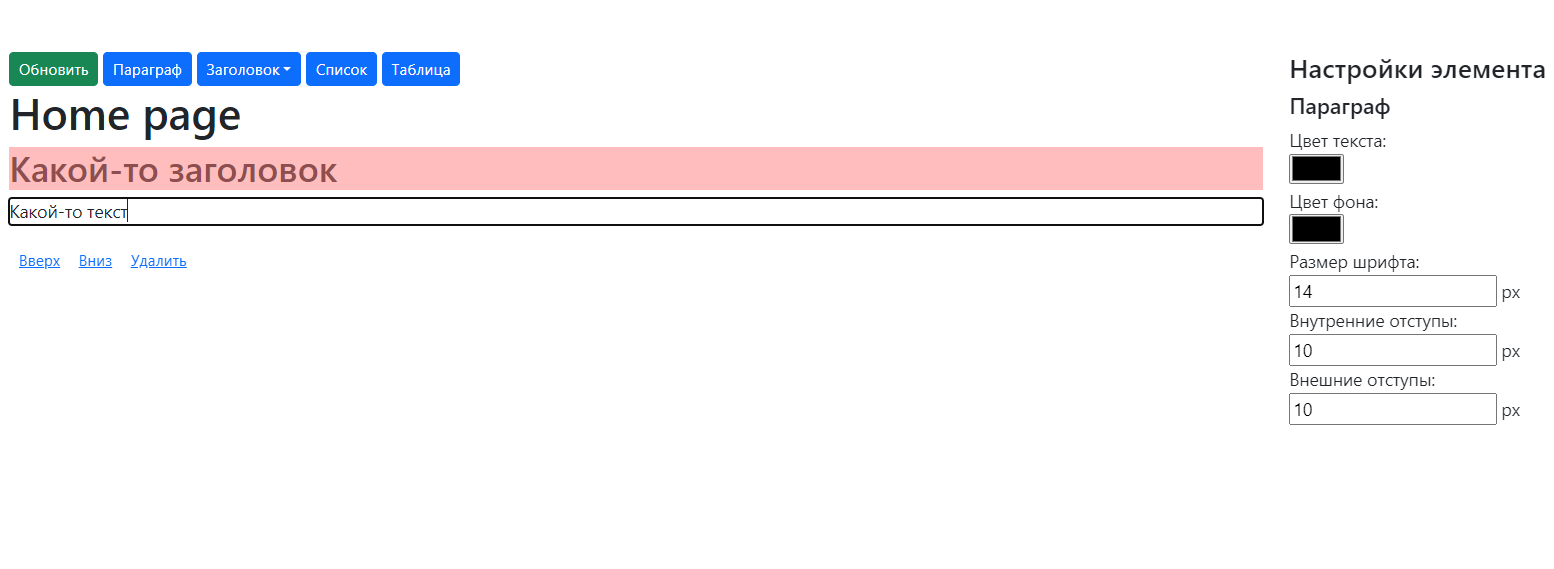
\includegraphics[width=1\linewidth]{ui10}}
	\caption{Редактор контента}
	\label{ui10:image}
\end{figure}

Внесенные изменения отображаюся на главной странице сайта (рис. \ref{ui11:image}).

\begin{figure}[H]
	\center{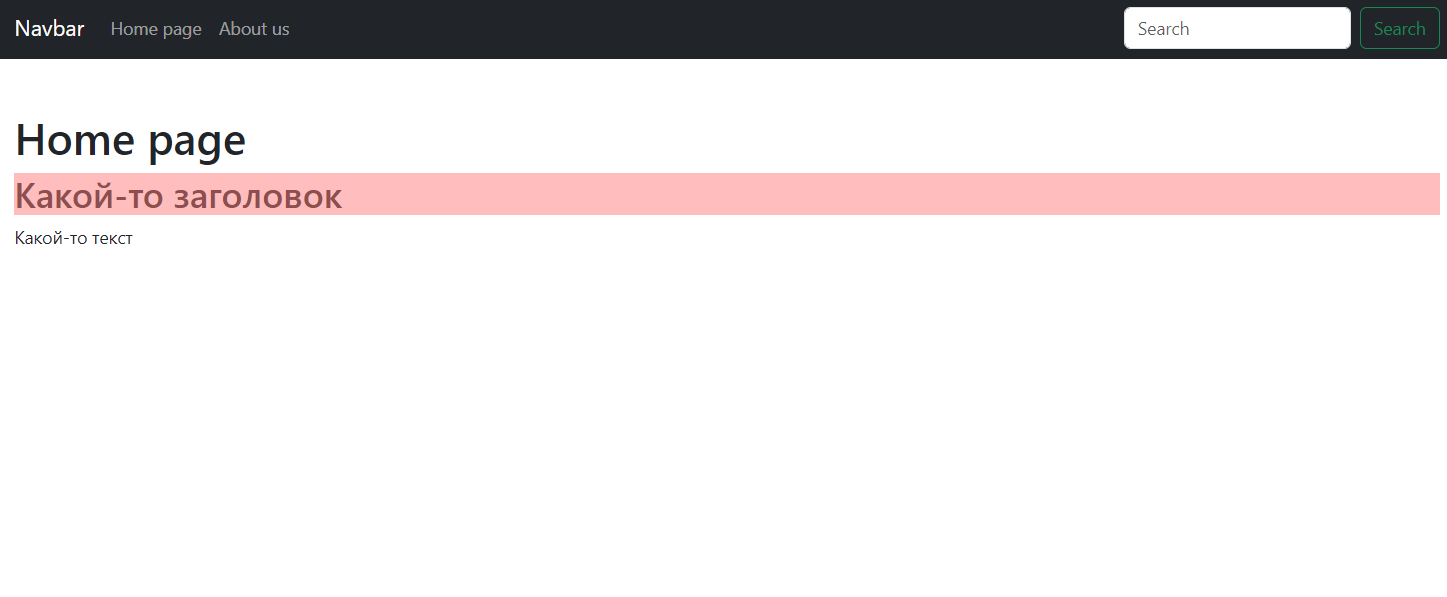
\includegraphics[width=1\linewidth]{ui11}}
	\caption{Главная страница сайта}
	\label{ui11:image}
\end{figure}

Для того чтобы управлять навигационными меню сайта, пользователю необходимо перейти в раздел "<Меню"> (рис. \ref{ui12:image}), в котором отобразиться список навигационных меню сайта.

\begin{figure}[H]
	\center{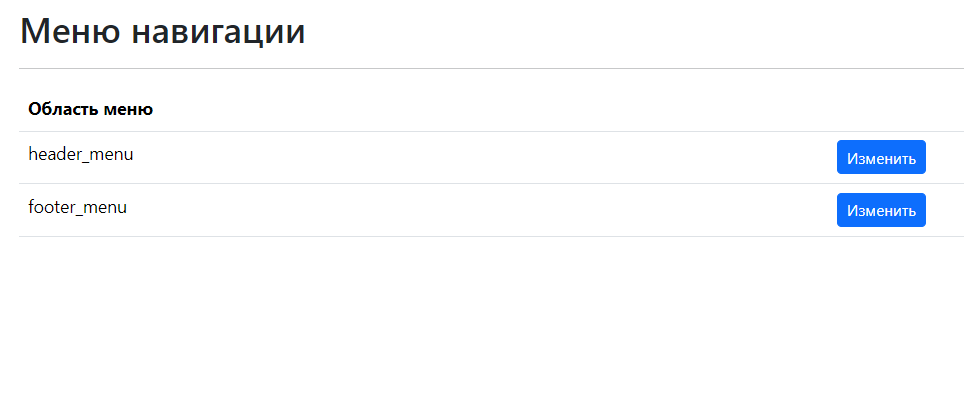
\includegraphics[width=1\linewidth]{ui12}}
	\caption{Список областей меню сайта}
	\label{ui12:image}
\end{figure}

Для добавление нового пункта меню, пользователь выбирает область меню, открывается страница со списком пунктов меню выбранной области меню (рис. \ref{ui13:image}), пользователь нажимает на кнопку "<Добавить">, появляется выпадающий список из опций: "<Страница">, "<Произвольная ссылка">. 

\begin{figure}[H]
	\center{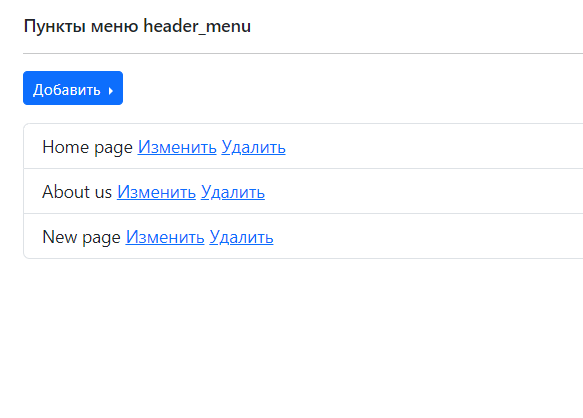
\includegraphics[width=1\linewidth]{ui13}}
	\caption{Список пунктов меню}
	\label{ui13:image}
\end{figure}

После выбора одной из опций появляется форма для добавления нового пункта меню (рис. \ref{ui14:image}).

\begin{figure}[H]
	\center{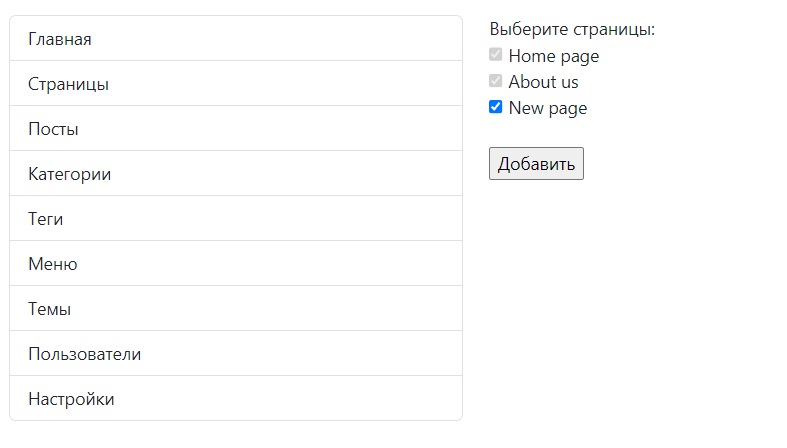
\includegraphics[width=1\linewidth]{ui14}}
	\caption{Форма добавления нового пункта меню}
	\label{ui14:image}
\end{figure}

После ввода данных пункта меню, при нажатии на кнопку "<Добавить">, новый пункт меню добавляется в меню и отображается в шапке сайта (рис. \ref{ui15:image}).

\begin{figure}[H]
	\center{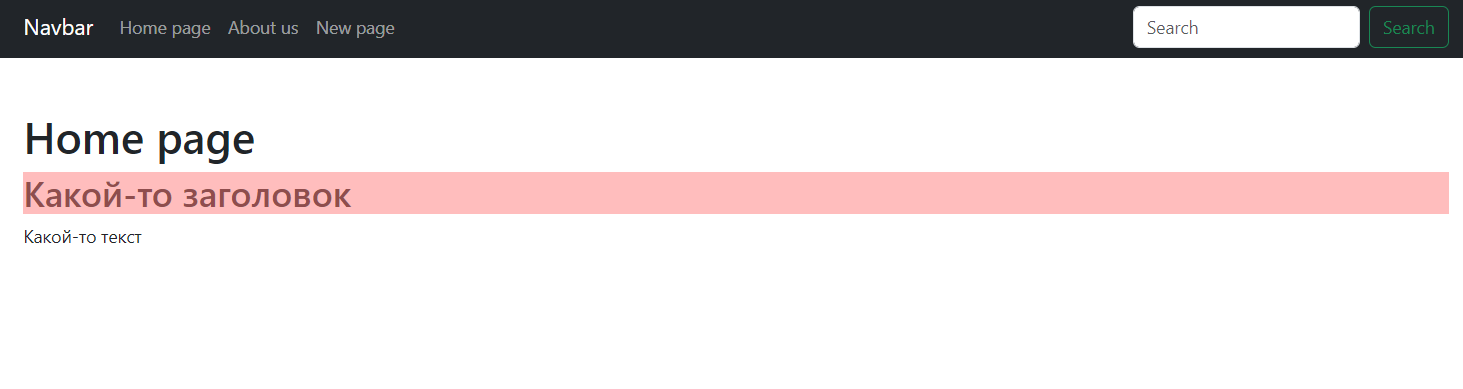
\includegraphics[width=1\linewidth]{ui15}}
	\caption{Добавленный пункт меню}
	\label{ui15:image}
\end{figure}
		
		
		
\subsection{Сборка компонентов программной системы}

Компоненты программно-информационной системы включают в себя файлы классов, скрипты, шаблоны страниц, ресурсы, библиотеки, конфигурационные файлы и прочие файлы, которые используются для функционирования системы.

Для компиляции и сборки всех программ, входящих в состав программно-информационной системы, необходимы установленный на компьютер HTTP-сервер и интерпритатор языка PHP.

Программная система запускается в браузере.

%На рисунке \ref{main:image} представлена главная страница сайта «Русатом – Аддитивные технологии».
%\newpage % при необходимости можно переносить рисунок на новую страницу
%\begin{figure}[H] % H - рисунок обязательно здесь, или переносится, оставляя пустоту
%\center{\includegraphics[width=1\linewidth]{main1}}
%\center{\includegraphics[width=1\linewidth]{main2}}
%\center{\includegraphics[width=1\linewidth]{main3}}
%\caption{Главная страница сайта «Русатом – Аддитивные технологии»}
%\label{main:image}
%\end{figure}

%На рисунке \ref{menu:image} представлен динамический вывод заголовков, включающий в себя искомые фразы при поиске фраз.

%\begin{figure}[ht]
%\center{\includegraphics[width=1\linewidth]{menu}}
%\caption{Динамический вывод заголовков}
%\label{menu:image}
%\end{figure}
%
%На рисунке \ref{enter:image} представлен ввод данных для публикации новости.
%
%\begin{figure}[ht]
%\center{\includegraphics[width=1\linewidth]{enter}}
%\caption{Ввод данных для публикации очень-очень длинной, интересной и полезной новости}
%\label{enter:image}
%\end{figure}
